\documentclass[12pt,a4paper,spanish]{book} 
\usepackage{babel}
\usepackage [T1]{fontenc}
\usepackage [latin1]{inputenc}
\usepackage{graphicx}
\usepackage{array}
	  \oddsidemargin 0in
      \textwidth 6.75in
      \topmargin 0in
      \textheight 10.0in
      \parindent 0em
      \parskip 2ex
\usepackage{anysize}
\marginsize{3cm}{2cm}{1.0cm}{1.0cm}

\pagestyle{plain}

\begin{document} 
\title{
\begin{table}[!h]
	\begin{tabular}{m{2cm}m{15cm}}
		\multicolumn{1}{l}{}
		 
\includegraphics[scale=0.25, bb=0 0 0 0]{images/logo-fiuba.png} & 
		 \begin{center}
		 	\begin{LARGE}
				Universidad de Buenos Aires	\linebreak \linebreak		 							Facultad de Ingenier\'{i}a  \linebreak \linebreak
				7112 - Estrucutra de las Organizaciones \linebreak \linebreak
				2do. Cuatrimestre de 2009
			\end{LARGE}
		 \end{center}\\
\end{tabular}
\end{table}
\begin{Large}
 \begin{center}
		\underline{Trabajo Pr\'{a}tico} \linebreak \linebreak
        Grupo Nro:	R2
\end{center}
\end{Large}
}
\date{}
\maketitle

\thispagestyle{empty}
\author{
\begin{Large}
\begin{center}
		\underline{Integrantes}  \linebreak 
\end{center}
\end{Large}
\begin{center}
	\begin{tabular}{|| c | c | c ||}
		\hline
		\begin{large}Apellido,Nombre\end{large} & 
		\begin{large}Padr\'{o}n Nro.\end{large} & 
		\begin{large}E-mail\end{large}\\
		\hline
		Bruno Tom\'as & 88449 & tbruno88@gmail.com\\
		\hline
		Chiabrando Alejandra Cecilia & 86.863 & achiabrando@gmail.com\\
		\hline
		Fern\'{a}ndez Nicol\'{a}s  & 88.599 & nflabo@gmail.com\\
		\hline
		Invernizzi Esteban Ignacio & 88.817 & invernizzie@gmail.com\\
		\hline
		Medbo Vegard & \- & vegard.medbo@gmail.com\\
		\hline
		Meller Gustavo Ariel & 88.435 & gustavo\_meller@hotmail.com\\
		\hline
		Mouso Nicol\'as & 88.528 & nicolasgnr@gmail.com\\
		\hline
		Mu\~noz Facorro Juan Mart\'in & 84.672 & juan.facorro@gmail.com\\
		\hline
		Wolfsdorf Diego & 88.162 & diegow88@gmail.com\\
		\hline
	\end{tabular}
\end{center}
}

\newpage

\setcounter{page}{1} 
\tableofcontents

\chapter*{Introducci�n}
\addcontentsline{toc}{chapter}{Introducci�n}

El presente trabajo apunta analizar la situaci�n actual de la filial argentina de la empresa Marsans Viajes. La misma se encuentra atravesando un per�odo de crisis, lo que la llev� a tomar distintas decisiones que repercutieron, no siempre de manera favorable, en su estructura. Con el fin de ayudar a la empresa a superar los problemas que atraviesa y ponerla nuevamente en el camino hacia el liderazgo de las agencias de viajes, se busc� individualizar los distintos problemas que presenta la empresa, poniendo �nfasis en aquellos de �ndole estructural. Se hizo un an�lisis de la repercusi�n de dichos problemas en el funcionamiento de la empresa y se presentan propuestas de cambio. 

\part{Casos de Estudio}

\chapter{Elevadores H�rcules}

\section{Historia de la Empresa}
Elevadores H\'{e}rcules S.A., se estableci\'{o} en Buenos Aires en 1919 como una oficina de contratistas.
Su planta principal est\'{a} ubicada en Buenos Aires. Adem\'{a}s tiene oficinas comerciales en las 18 ciudades m\'{a}s importantes del pa\'{i}s participando con m\'{a}s del 60 \% del mercado nacional.

\subsection{Avance Cronol\'{o}gico de la empresa}
\begin{enumerate}
	\item \underline{1966}. La compa\~{n}\'{i}a produc\'{i}a 1650 elevadores. 
	\item \underline{1970}. Hacia esta d\'{e}cada el n\'{u}mero de edificios comenz\'{o} a aumentar considerablemente. Los pedidos de los clientes tend\'{i}an a sobrepar la capacidad de producci\'{o}n de la f\'{a}brica.
	\item \underline{1974}. Lleg\'{o} a producir 7.850 unidades, inclusive escaleras mec\'{a}nicas.
\end{enumerate}

\section{Resumen del Funcionamiento}

\subsection{Caracter\'{i}sticas del Sistema de Producci\'{o}n}
\begin{itemize}
	\item \emph{No} depende de proveedores para la fabricaci\'{o}n de los productos, es decir, la misma es vertical. La empresa no terceriza nada sino que todo lo produce ella misma. Con lo cual toda la producci\'{o}n es propia.
	\item Producci\'{o}n diversificada debido a lo anterior, dando lugar a un complejo sistema de producci\'on en general.
	\item Producci\'{o}n no estandarizada, debido a los diversos requerimientos de los clientes. Cuenta con pocas piezas estandarizadas.
	\item El planeamiento tambi\'{e}n est\'a dificultado por el desarrollo tecnol\'ogico de la construcci\'on de diferentes lugares, dependiendo as\'i de condiciones que no se pueden preveer. Al producir todo la misma empresa el planeamiento se torna dificultoso, ya que no solamente se construye el elevador sino que tambien se tienen que construir todas las piezas del mismo, lo que hace que la planificaci\'{o}n tambi\'{e}n incluya la construcci\'{o}n de las piezas. Otro punto que dificulta el planeamiento es que no se tiene una estandarizaci\'{o}n de los procesos con lo que al no producir estandarizado se tiene que planear todo el tiempo distintas cosas lo cual aumenta el margen de error, teniendo probabilidades m\'{a}s grandes de ineficiencia.
	\item Equipo de producci\'{o}n y montaje dividido en 4 grupos(seg\'{u}n la secuencia en el orden de entrega de partes.)
	\item Producci\'{o}n organizada por secciones:
	\begin{enumerate}
		\item M\'{a}quinas operativas.
		\item Estampado.
		\item Montaje de m\'{a}quinas.
		\item Montaje de motores
		\item Montaje de aparatos el\'{e}ctricos.
		\item Montaje y conexi\'{o}n de cuadros de comando.
		\item Carpinter\'{i}a, fabricaci\'{o}n de contrapesos, cabinas y 	puertas de acero.
		\item Carpinter\'ia, cabinas, puertas y plataformas de madera.
		\item Pintura y galvanoplast\'ia.
	\end{enumerate}
	\item Proceso de Planeamiento de Producci\'{o}n
	\begin{itemize}
		\item El equipo de producci\'{o}n y montaje de elevadores estaba formado en grupos.
		\item Cada grupo responsable de una tarea diferente.
		\item El Jefe de grupo estimaba futuras necesidades, volcando esto en un formulario de avances del mes, donde planificaba adem\'{a}s tiempos de entrega seg\'{u}n el proceso de producci\'{o}n mencionado antes.
		\item  Se entregaba el formulario a un asistente(planeador) del Departamento de Producci\'{o}n.
		\item El planeador con dichos formularios, elabora el programa de producci\'{o}n siguiendo una secuencia impuesta por el Departamento de Ventas(orden de entrada de los pedidos de los clientes)
		\item El planeador tambi\'{e}n recibe ordenes de fabricaci\'{o}n individuales del Departamento de Ingenier\'{i}a, que contiene las especificaciones para producir el elevador.
	\end{itemize}
	\item Cuando la cantidad de elevadores producidos era baja comparada con la capacidad de producci\'{o}n el planeamiento era simple,eficaz y de f\'{a}cil control. 
	\item Hacia 1970, los retrasos en las entregas hacian que:
	\begin{itemize}
		\item Jefes de campo fijaran plazos muy anticipados, haciendole perder el valor agregado del programador.
		\item Falla en la comunicaci\'{o}n al momento de la par\'{a}lisis de las obras de un edificio, produciendo estancamiento de stock y as\'{i} generando grandes atrasos y malestar de los clientes.
		\item Por todo esto el Departamento de Ventas sugiri\'{o} cambios en las prioridades de las ordenes de producci\'{o}n
		\item Se abandon\'{o} la programaci\'{o}n que se llevaba hasta ese momento, dependiendo de las ordenes de venta del Departamento respectivo.
	\end{itemize}
\end{itemize}

\newpage
\section{Organigrama tentativo}
Se detalla un organigrama parcial que se confecciona a partir de la informaci\'on proporcionada en la descripci\'on del caso.

\begin{figure}[H]
\centering
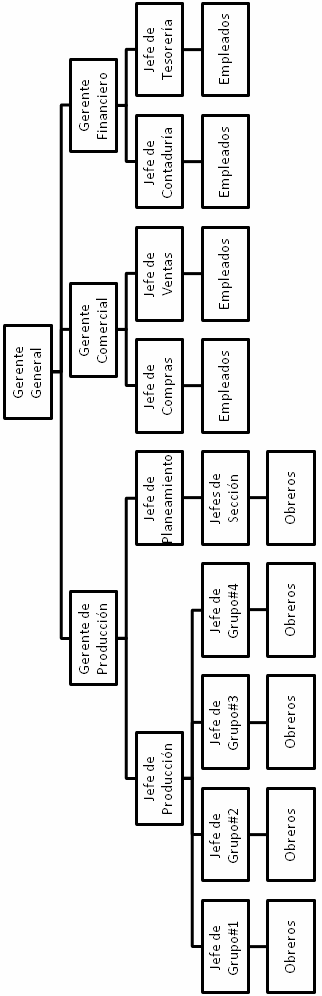
\includegraphics[scale=0.75]{images/organigrama-hercules.png}
\end{figure}

\newpage
\section{An\'{a}lisis del caso}

\subsection{Marco Te\'orico}

\subsubsection{Tipo de empresa}
La empresa fue en sus comienzos probablemente una PyME, y a medida que aument\'o su tama\~no desarroll\'o su vida como una sociedad civil. En este sentido, si bien nunca fue una empresa familiar, su estructura y organizaci\'on iniciales fueron evolucionando gradualmente a lo que es en la actualidad, probablemente provocando los problemas de planeamiento observados. Es decir, si una empresa no sufre un proceso formal de dise\~no organizacional, es altamente probable que se encuentren deficiencias en su funcionamiento a medida que pasa el tiempo y aumenta su tama\~no. Por este motivo resulta conveniente la reestructuraci\'on que se propone la empresa al contratar una consultora.

\subsubsection{Proceso de creaci\'on de valor}
Una observaci\'on interesante es el amplio proceso de conversi\'on de insumos en productos. La empresa toma como insumos materias primas muy esenciales, para utilizar en fundici\'on, carpinter\'ia, torner\'ia, moldeado, rectificaci\'on, montaje, pintura, estampado y la final instalaci\'on de los productos. Una empresa de esta complejidad necesita una estructura s\'olida y una programaci\'on muy precisa para funcionar eficientemente.

\subsubsection{Rasgos de pensamiento administrativo}
Evidentemente la empresa evolucion\'o hacia el modelo de Taylor: en un principio delegaba en los empleados parte del planeamiento de producci\'on, quienes reportaban al planeador de producci\'on, que luego completaba la programaci\'on. Esto trajo problemas por dos motivos; uno de ellos los errores de relevamiento de dichos empleados, quienes omit\'ian reportar obras paralizadas y fijaban plazos de entrega muy anticipados para tratar de compensar los retrasos en las entregas (meti\'edose en una parte de la organizaci\'on que no era su responsabilidad); el otro motivo fue el aumento de la demanda, que hizo imposible continuar con este precario sistema. Se pasa entonces a trabajar seg\'{u}n ordenes de venta, lo cual hace el negocio menos previsible (quita la posibilidad reaccionar ante fluctuaciones en el mercado, la programaci\'on se hace a medida que se vende pero no se pronostica la potencial demanda futura).

\subsection{Problema principal de la empresa}
\subsubsection{La empresa no puede enfrentar al cambio en el mercado}
El problema principal de H\'ercules surge al producirse un cambio en el mercado. La empresa comienza atendiendo a una cantidad de clientes con la cual puede trabajar en forma eficiente y c\'omoda. Al empezar a irle bien cada vez cuenta con m\'as clientes y m\'as pedidos. Esto deber\'ia serle algo muy positivo a la misma, ya que le implicar\'ia ganar m\'as que antes y ampliar su mercado. Pero esto no es lo que sucede ya que, contrario a lo que se supone como un crecimiento, es aqu\'i cuando empiezan los problemas.\\

\subsection{Consecuencias del problema principal de la empresa y sus propuestas de soluci\'on}

\subsubsection{No hay una determinaci\'on de que procesos dan valor y cuales no}
La empresa es dif\'icil de controlar y no logra una correcta planificaci\'on, debido a que su proceso productivo es muy amplio y abarcativo. De un an\'alisis de los procesos industriales de la empresa puede reconocerse una falencia: hay procesos que no agregan valor al producto final. Es decir, la empresa realiza tareas como la fabricaci\'on de las piezas a utilizar en la construcci\'on de los elevadores, las cuales podr\'ian ser compradas a terceros. Como se mencionar\'a m\'as adelante, la fabricaci\'on de las piezas tambi\'en representa un costo innecesario.
\paragraph{Soluci\'on}
Se debe determinar qu\'e procesos que agregan valor y los que no, y a partir de all\'i tomar decisiones en la direcci\'on de abandonar los procesos que no producen un beneficio a la empresa, ya sea directo o indirecto (ventajas competitivas, por ejemplo), y si este beneficio justifica el costo del proceso. Un claro ejemplo de proceso que agrega valor en la empresa es el dise\~no y construcci\'on de elevadores. Este es un trabajo que la empresa transforma directamente en ingresos, ya que es su actividad principal. Un ejemplo de proceso que no agrega valor es el de la fabricaci\'on de piezas est\'andar: ellas pueden ser compradas a un tercero, y probablemente adem\'as se reduzca su costo, ya que el tercero puede producirla en mayor cantidad, y la empresa deber\'ia podr\'ia abandonar los costos fijos asociados a su producci\'on.

\subsubsection{Grave problema de costos}
La empresa tiene un grave problema de costos, algunos de ellos ocultos tras otros problemas. Se encuentra desbordada de pedidos y no tiene una respuesta eficiente; para intentar hacerles frente a los mismos toma decisiones equivocadas y principalmente apresuradas. Intentar vender m\'as en este caso no le esta garantizando mayor ganancia ya que en alg\'un momento esta situaci\'on de toma de decisiones erroneas va a hacer que el rendimiento comience a bajar notoriamente. Las principales decisiones erroneas son:
	\begin{itemize}
 		\item Coloca personal incapacitado para ciertos puestos. 
		\item No tiene un control efectivo de lo que produce, puede estar produciendo piezas equivocadas o m\'as de lo que realmente necesita ya que no cuenta con un plan eficaz. Esto se traduce en un costo de almac\'en porque debe acumular stock de piezas.
		\item Acepta cualquier pedido sin saber si realmente llega a cumplimentarlo, por una descoordinaci\'on entre el \'area de ventas y el \'area de producci\'on.
		\item Construye cada elevador a medida del cliente lo cual perjudica la producci\'on ya que no est\'a estandarizada, lo cual hace que aumente el margen de error (costos de reparaci\'on y/o reemplazo), agrega un costo de dise\~no a cada proyecto, agrega un costo de servicio de venta personalizado, etc.
	\end{itemize}
\paragraph{Soluci\'on}
Para el problema de costos una posible soluci\'on es estandarizar los procesos de producci\'on, y establecer un nuevo proceso de selecci\'on de personal, al menos del jer\'arquico.\\
Deben dise\~narse una serie de modelos est\'andar determinando antes cu\'ales son las caracter\'isticas de los elevadores m\'as vendidos, armar un catalogo para ofrecer a los clientes y fabricar los productos en serie. De esta manera es posible disminuir al menos dos costos: el de dise\~no, que no debe repetirse para cada cliente, y el de producci\'on o compra de piezas, ya que se estandarizar\'an completamente. Con esto podr\'ia llegar a perder una parte del mercado, pero consideramos que no ser\'{a} una gran parte ya que los productos a medida en general son m\'as costosos que los est\'andar, y los productos menos costosos son los que consiguen mayor caudal de ventas.\\
Se propone que el proceso de fabricaci\'on de piezas sea tercerizado, con esto bajar\'a la dificultad del planeamiento, se tendr\'{a} un menor sector de producci\'on m\'{a}s controlable, m\'as eficiente. Disminuir\'an notablemente los costos de dep\'osito, el costo de la planificaci\'on, se reducir\'a tambi\'en el costo de las piezas, ya que al ser est\'andar habr\'a m\'as de un proveedor compitiendo con sus precios por abastecer a la empresa.\\
Para lograr este tipo de decisiones debe contratarse personal capacitado para la planificaci\'on de una empresa de la escala de H\'ercules, si es posible con experiencia en el \'area de las instalaciones en la construcci\'on, por lo menos un director o gerente de planeamiento de producci\'on que posea mayores conocimientos que los t\'ecnicos de este \'area, para poder ejercer una autoridad real. Puede establecerse un \'area de recursos humanos para definir pol\'iticas de reclutamiento apuntadas a este objetivo, o contratarse una agencia consultora de forma temporal si no se requieren tareas de RR.HH. continuas.

\subsubsection{Falta de estandarizaci\'on, diversidad de productos}
La empresa se maneja en un ambiente muy cambiante, donde las variables externas (que no son controlables) son abundantes: los productos no son est\'andar, por ello no hay plan general de producci\'on (por la particularidad de cada producto vendido); el desarrollo tecnol\'ogico de la construcci\'on var\'ia segn el lugar de instalaci\'on de cada productos, etc.
\paragraph{Soluci\'on}
La empresa necesita un vuelco hacia el enfoque de contingencias, para adaptar las variables administrativas a las externas (que no son controlables.) En este sentido, se debe verificar que el personal administrativo cuente con el alcance temporal de la discreci\'on adecuado. Se debe adem\'{a}s analizar el ambiente externo produciendo informaci\'on confiable para reducir el riesgo en la toma de decisiones. Por ejemplo, contratar una consultora, o abrir una nueva \'area de la empresa, dedicada a la estad\'istica y pron\'osticos de mercado.

\subsubsection{Contrataci\'on de personal no capacitado para las tareas requeridas}
Se nombr\'o a cargo del Planeamiento de la Producci\'on a un antiguo supervisor en 1942. El nombramiento de esta persona no cumple con los requisitos del alcance temporal de la discreci\'on. Esto quiere decir que la persona no tiene la capacidad de predecir o anticipar el desarrollo de la tarea en el lapso de tiempo adecuado para tomar decisiones de planeamiento. Esto se ve reflejado en el siguiente parrafo de la descripci\'on del caso: "Los retrasos en las entregas de elevadores hicieron que los jefes de campo fijasen los plazos de entrega muy anticipados en sus informes mensuales. Con eso las informaciones recibidas por el programador, fueron perdiendo parte de su valor como base para la programaci\'on."\ Al meter personas en lugares equivocados no se soluciona nada sino que se empeora la situaci\'on. La empresa quiza quiera ahorrarse alg\'un costo de traer a un profesional, pero a la larga tiene m\'as costo por no traerlo.
\paragraph{Soluci\'on}
Se propone situar en ese cargo a una persona que cumpla con los requerimientos que la posici\'on requiere. Alguien con experiencia y previsi\'on, que sea capaz de coordinar tiempos y tareas junto con el Area de Produccion.

\subsubsection{Conflictos entre algunas \'areas de la empresa}
"Los pedidos de los clientes tend\'ian a alcanzar l\'imites que sobrepasaban la capacidad de producci\'on de la f\'abrica. Los atrasos en la entrega de pedidos llegaron al punto de provocar serios conflictos entre los departamentos de ventas y producci\'on."
\paragraph{Soluci\'on}
Se propone incluir alg\'un tipo de nexo entre ambos departamentos. No puede pasar que el departamento de ventas y de producci\'on no se comuniquen ya que lo que se produce es lo que se vende, no se puede vender algo que no se va a poder producir. La gente de ventas no tiene el m\'as m\'inimo conocimiento de como se produce (lo cual es correcto ya que su funci\'on no es producir, sino vender) por lo que no tiene una noci\'on exacta de tiempos. Por lo que si no hay alguien que actue de nexo entre ambas \'areas, nunca va a funcionar bien. Encima una empresa vive de lo que vende por lo que este es un punto realmente importante. Creemos que ser\'ia correcto crear una relaci\'on formal entre la gerencia de ventas y la gerencia de producci\'on para que se pueda trabajar a conciencia de tiempos y no se produzcan conflictos entre ambas \'areas.

\subsubsection{Demasiadas tareas de producci\'on}
La diversificaci\'on de producci\'on produce gran parte del colapso del sistema, dado que se quiere abarcar gran cantidad de tareas de producci\'{o}n que no son pertinentes al objetivo de la empresa que es dise\~nar, construir e instalar elevadores. Sin embargo tiene la ventaja de tener capacidad de producci\'on propia y no depender de terceros, lo cual resulta interesante sobre todo cuando se trata de piezas no estandarizadas.
\paragraph{Soluci\'on}
Aqu\'i es cuando aparecen dos posibles soluciones: La primera es tercerizas la producci\'on de partes est\'andar. La contrapartida a esta soluci\'on es mejorar la programaci\'on para permitir el correcto funcionamiento del \'area de producci\'on, salvando el problema sin cerrar los talleres que producen las partes est\'andar. 
Podemos analizar los distintos costos de ambas alternativas:
Al tercerizar la fabricaci\'on debe cerrarse un \'area de la empresa, debiendo prescindir de empleados de varios niveles, o mantenerlos en otro \'area de la empresa aumentando los costos de mano de obra; se perder\'ia parte de la inversi\'on en capacidad productiva de partes est\'andar, ya que seguramente ser\'a dif\'icil vender maquinaria especializada usada. En contrapartida puede ser mejor al trabajar con un planeamiento m\'as chico, se puede tener un mejor control sobre la producci\'on verdadera de la empresa (que son los elevadores), se reduce el costo de calidad y eso puede hacer que se reduzca el costo de fabricaci\'on. No siempre al fabricar uno las piezas se garantiza el menor costo, muchas veces adquiriendolas de un tercero el mismo es menor.
El mejorar la programaci\'on conlleva costos de reorganizaci\'on en t\'erminos de personal administrativo para sostener un proceso burocr\'atico m\'as funcional que el actual; tal vez sea necesario una actualiaci\'on de los sistemas de informaci\'on de la empresa, lo cual puede ser un costo bastante alto.
Para mejorar la programaci\'on de la producci\'on podr\'ia adoptarse un cronograma como el propuesto a continuaci\'on:
\begin{enumerate}
\item Se realiza un pedido de instalaci\'on desde una obra.
\item Se analiza qu\'e partes son est\'andar y cu\'ales no (a cargo del Departamento de Ingenier\'{i}a a trav\'es del formulario de fabricaci\'on individual).
\item Las partes est\'andar se solicitan a las empresas tercerizada (por el Departamento de Compras).
	\begin{itemize}
		\item Tener en cuenta que es conveniente contar con una red de proveedores, por si uno no puede producir que otra pueda hacerse cargo de una mayor parte de la producci\'on.
	\end{itemize}
\item Teniendo en cuenta el tiempo de fabricaci\'on propio (ensamble de partes, creaci\'{o}n de las propias, etc.) m\'as el de la entrega de las partes no comunes, se elaborar\'{a} el informe para la obra.
\item En caso de par\'{a}lisis de obra, se evaluar\'{a} el tiempo del mismo, y se intentar\'ia la redistribuci\'{o}n de los semielaborados comunes en otras obras.
\item Todas las semanas se confeccionar\'an informes del avance de cada obra en que se ha encargado una instalaci\'on.
\item El Departamento de Ventas solo debe encargarse de la venta en s\'i y de los requerimientos iniciales, sin interferir en el resto del proceso.
\end{enumerate}

\section{Historia de la Empresa}
	S-S Technologies Inc. se constituy\'{o} en 1992 cuando la  compa\~{n}\'{i}a constructora y de ingenier\'{i}a integrada Sutherlaud- Schultz, de la cual formaba parte, cambi\'{o} de propietarios y los nuevos due\~{n}os vendieron la parte de SST al ex presidente de Sutherlaud- Schultz, Brock. La compa\~{n}\'{i}a era de  propiedad 100 por ciento canadiense. En \'{u}ltima instancia, SST era propiedad de su director general, Rick Brock, ex presidente de Sutherland-Schultz, y de Keith Pritchard, presidente de SST. 
	En enero de 1994 la compa\~{n}\'{i}a enfrentaba un r\'{a}pida tasa de crecimiento que se estimaba pod\'{i}a duplicarse o triplicarse en los dos a\~{n}os siguientes. En los \'{u}ltimos 3 a\~{n}os se hab\'{i}a percibido un crecimiento promedio de 33 por ciento anual y se esperaba un crecimiento de 30 a 60 o incluso 120 empleados.

	\subsection{Avance Cronol\'{o}gico de la empresa}
	\begin{enumerate}
		\item \underline{1992}. Se constituye la compa\~{n}\'{i}a al venderse la parte correspondiente a Brock. 
		\item \underline{1993}. Se perciben ingresos por 6.3 millones de d\'{o}lares.
		\item \underline{1994}. Se estima un crecimiento que duplique o triplique al del a\~{n}o anterior.
	\end{enumerate}

\section{Resumen del Funcionamiento}

	\subsection{Caracter\'{i}sticas del Sistema de Producci\'{o}n}
	\begin{itemize}
		\item La p oducci\'{o}n se divide en dos grupos: productos y sistemas integrados:
		\begin{enumerate}
			\item Productos participaba del desarrollo y venta de productos de hardware y sofware propios de la compa\~{n}\'{i}a, los cuales se vend\'{i}an por todo el mundo. Los mismos comprend\'{i}an las tarjetas simuladoras Direct-Link y el simulador PICS, los cuales peresentaban una soluci\'{o}n a un problema que ninguna otra compa\~{n}\'{i}a pod\'{i}a resolver.
			\item El grupo de sistemas integrados trabajaba en tres \'{a}reas distintas pero interrealacionadas: consultor\'{i}a, ingenier\'{i}a de sistemas y soporte a clientes brindando soluciones de calidad a problemas de hardware y software a complejos sistemas de pisos de f\'{a}bricas.
			\end{enumerate} 
		\item Ante la recesi\'{o}n, la compa\~{n}\'{i}a se ve beneficiada ya que brinda soluciones que permiten reducir los costos de automatizaci\'{o}n de las plantas y por ende los costos de producci\'{o}n.
		\item Se ten\'{i}a un enfoque de consultor\'{i}a que permit\'{i}a que quienes participaban tuvieran facultades de decisi\'{o}n y llevaba a apropiarse de los problemas y sus soluciones.
		\item Los proyectos eran asignados a individuos o equipos, seg\'{u}n el tama\~{n}o, los cuales eran autoadministrados. La responsabilidad de los proyectos reca\'{i}a en los integrantes del grupo generando un alta motivaci\'{o}n.
		\item La organizaci\'{o}n era austera, manteniendo los recursos indirectos al m\'{i}nimo.
		\item El principal recurso de la empresa lo representaba su capital humano formado de equipos muy competentes, t\'{e}cnicos y motivados. El personal t\'{e}cnico era l\'{i}der en su campo.
		\item Otro recurso era su excelente reputaci\'{o}n y relaci\'{o}n con un gran fabricante canadiense.
		\item La empresa estaba adelantada en la curva de apredizaje, habiendo enfrentado varios desaf\'{i}os, los cuales pudo resolver con \'{e}xito.
	\end{itemize}

\newpage
\section{An\'{a}lisis del caso}

	\subsection{Marco Te\'orico}

		\subsubsection{Dise\~{n}o administrativo}
			Si bien tiene un organigrama definido, la mayor parte de las relaciones que se dan en la misma son de car\'{a}cter informal. Se conforman grupos de trabajo con mecanismo coordinador de ajuste mutuo sobre los que recae la responsabilidad de las tareas que llevan a cabo. La forma de reportar no respeta el organigrama sino que se da de acuerdo a relaciones informales o costumbre.

		\subsubsection{Rasgos de pensamiento administrativo}
			La empresa presta especial atenci\'{o}n a las ciencias del comportamiento. Se busca que todos los empleados participen y sientan que todas sus necesidades se encuentran satisfechas a la vez que se valora la motivaci\'{o}n y el compromiso. Las relaciones informales cobran especial importancia con el sistema de comunicaci\'{o}n abierto que se implementa.

	\subsection{Problemas de la empresa y sus respectivas soluciones}


		\subsubsection{Falta de claridad en las metas y estrategias de la empresa}
			Los empleados no tienen en claro las metas y estrategias de la empresa. 
			Las funciones y responsabilidades de los distintos puestos resultan confusas.
			El abuso de las relaciones informales y poco respeto al organigrama genera que los empleados no reporten a quien deber\'{i}an creando caos. 
		\paragraph{Soluci\'on}
			Deber\'{i}a utilizarse un enfoque burocr\'{a}tico a fin de definir la autoridad, funciones y responsabilidades de los distintos puestos y dejar en claro la jerarqu\'{i}a de los cargos. 
			Aquellas personas en puestos de autoridad deber\'{i}an exigir que se cumplan estas relaciones. 
			Es necesario designar formalmente un gerente para el Grupo de Productos y otro para el Grupo de Sistemas Integrados. 
			Esto puede traer un conflicto interno dentro del grupo GSI  pero es necesario para resolver las confusiones que tienen los integrantes del grupo en lo que respecta a la autoridad de Shwarz respecto a Ojala.
		
		\subsubsection{Falta de espacio f\'isico}
			La compa\~{n}\'{i}a hab\'{i}a crecido tanto que resultaban insuficientes las instalaciones que compart\'{i}a con otras empresas. Como no se quer\'{i}a separar al personal, se agreg\'{o} un remolque para ubicar al personal adicional.
		\paragraph{Soluci\'on}
			Una alternativa es la b\'{u}squeda de un edificio con mayor disponibilidad de instalaciones a fin de que todos los empleados puedan trabajar en un lugar c\'{o}modo sin que sea necesaria la divisi\'{o}n del mismo. 
			Existe una segunda alternativa que es reubicar a la otra empresa del dueo de SST, SAF o esperar a la culminaci\'{o}n  o rescindir el pr\'{e}stamo con la empresa Wilson Gas. 
			La ventaja de la primera alternativa es que la empresa no tendr\'{i}a que rescindir ning\'{u}n contrato ni tratar con otra empresa. 
			Adem\'{a}s se podr\'{i}a buscar un espacio que se adecue mejor a determinadas necesidades que despu\'{e}s de a\~{n}os en la producci\'{o}n, se identifican f\'{a}cilmente. 
			Las ventajas de la segunda alternativa es que la empresa no atravesar\'{i}a una mudanza en un momento en el cual, como muestra el caso, se espera una escasez de recursos y que como consecuencia se necesitar\'{i}a que todo recurso existente este abocado a satisfacer las necesidades del mercado sin perder tiempo en una mudanza.

		\subsubsection{No hay una figura que realice una tarea de recursos humanos}
			No se registran las evaluaciones de desempe\~{n}o y no existe una figura a la cual se le puedan hacer consultas referidas a los l\'{i}mites salariales de los diversos puestos.
		\paragraph{Soluci\'on}
			Creaci\'{o}n de un \'area de recursos humanos para que pueda guardar registro de las evaluaciones de desempe\~{n}o y que adem\'{a}s sirva para que los empleados puedan hacer consultas no t\'{e}cnicas sin sentirse inc\'{o}modos por tener que realizar la consultar a un superior.  

		\subsubsection{Falta de incentivo salarial a los empleados}
			Conflicto generado por ausencia de bonos y compensaciones. Los empleados no tienen un incentivo o un dinero extra por el trabajo realizado, con lo cual esto puede generar conflictos futuros (y no tan futuros) con los empleados.
		\paragraph{Soluci\'on}
			Se propone que la empresa realice evaluaciones individuales de performance del personal. 
			Para esto es necesario que se defina y respete un organigrama a fin de que quede en claro qui\'{e}n estar\'{a} siendo evaluado por qui\'{e}n. 
			Los mismos solo deberan premiar un excelente desempe\~{n} y preferentemente ser entregados a equipos de personal a fin de fomentar la cooperaci\'{o}n y limitar la competencia interpersonal. 
			Tambi\'{e}n debe considerarse entregar premios adicionales por contribuciones excepcionales.
			Los gerentes de cada \'{a}rea notificar\'{i}an al \'{a}rea de recursos humanos de los resultados de las evaluaciones t\'{e}cnicas para que este \'{a}rea sea la encargada de entregar los bonos y premios.
			Sera una funci\'{o}n del \'{a}rea de recursos humanos estudiar el estado econmico de cada empleado para analizar si es viable dar en forma de bonificaci\'{o}n acciones de la empresa para poder aumentar el sentimiento de pertenencia que siente cada empleado.


		\subsubsection{R\'apido crecimiento}
			Inminente crecimiento de la empresa en el corto plazo. La empresa en un per\'iodo corto de tiempo implement\'o un crecimiento importante, el 				cual fue demasiado r\'apido e hizo que se deban adaptar muchas cosas, algunas en forma eficiente y otras en forma ineficiente.
		\paragraph{Soluci\'on}
			Considerando que la empresa cuenta con mano de obra muy calificada es necesario ir contratando empleados para poder capacitarlos adecuadamente. 
			Teniendo en cuenta que la capacitaci\'{o}n implica que los empleados actuales destinen horas de producci\'{o}n e investigaci\'{o}n a la capacitaci\'{o}n de los nuevos empleados, la contrataci\'{o}n de personal deber\'{a} hacerse de a poco para que la producci\'{o}n no se vea comprometida.

\documentclass[12pt,a4paper,spanish]{article}
\usepackage[spanish]{babel}

\usepackage[ansinew]{inputenc}


\usepackage{graphicx}
\usepackage{float}
\usepackage{array}
	  \oddsidemargin 0in
      \textwidth 6.75in
      \topmargin 0in
      \textheight 10.0in
      \parindent 0em
      \parskip 2ex
\usepackage{anysize}
\marginsize{3cm}{2cm}{1.0cm}{1.0cm}

\pagestyle{plain}

\begin{document} 
\title{
\begin{table}[!h]
	\begin{tabular}{m{2cm}m{15cm}}
		\multicolumn{1}{l}{}
		 
\includegraphics[scale=0.5, bb=0 0 0 0]{logo-fiuba.png} & 
		 \begin{center}
		 	\begin{LARGE}
				Universidad de Buenos Aires	\linebreak \linebreak		 							Facultad de Ingenier\'{i}a  \linebreak \linebreak
				7112 - Estrucutra de las Organizaciones \linebreak \linebreak
				2do. Cuatrimestre de 2009
			\end{LARGE}
		 \end{center}\\
\end{tabular}
\end{table}
\begin{Large}
 \begin{center}
		\underline{An\'{a}lisis Caso Ford} \linebreak \linebreak
        Grupo Nro:	R2
\end{center}
\end{Large}
}
\date{}
\maketitle

\thispagestyle{empty}

\author{
\begin{Large}
\begin{center}
		\underline{Integrantes}  \linebreak 
\end{center}
\end{Large}
\begin{center}
	\begin{tabular}{|| c | c | c ||}
		\hline
		\begin{large}Apellido,Nombre\end{large} & 
		\begin{large}Padr\'{o}n Nro.\end{large} & 
		\begin{large}E-mail\end{large}\\
		\hline
		Bruno Tom\'as & 88.449 & tbruno88@gmail.com\\
		\hline
		Chiabrando Alejandra Cecilia & 86.863 & achiabrando@gmail.com\\
		\hline
		Fern\'{a}ndez Nicol\'{a}s  & 88.599 & nflabo@gmail.com\\
		\hline
		Invernizzi Esteban Ignacio & 88.817 & invernizzie@gmail.com\\
		\hline
		Medbo Vegard & \- & vegard.medbo@gmail.com\\
		\hline
		Meller Gustavo Ariel & 88.435 & gustavo\_meller@hotmail.com\\
		\hline
		Mouso Nicol\'as & 88.528 & nicolasgnr@gmail.com\\
		\hline
		Mu\~noz Facorro Juan Mart\'in & 84.672 & juan.facorro@gmail.com\\
		\hline
		Wolfsdorf Diego & 88.162 & diegow88@gmail.com\\
		\hline
	\end{tabular}
\end{center}
}

\newpage
\setcounter{page}{1}
\tableofcontents

\newpage

\section{Introducci�n}
	Para el �xito de una empresa, es indispensable que �sta conozca su ambiente y se sepa adaptar al mismo.
	No basta �nicamente con cerrar tratos convenientes con los clientes, sino que tambi�n hace falta considerar otras variables, como por ejemplo los proveedores y la competencia.
	El conjunto de todas estas variables forma lo que se conoce como el ambiente.

	Formalmente, el ambiente se puede definir como el sistema de nivel superior en el que se inserta la empresa y est� formado por aquellos factores, fuerzas o variables que influyen directa, o indirectamente, en los procesos de gesti�n\cite{ITE}.
	El conocimiento de una empresa de su ambiente le permite explotar al m�ximo su potencial e incluso poder anticiparse a situaciones riesgosas.

	La empresa Ford Motor Company  se fund� a principios del siglo XX.
	Ya desde sus comienzos se dedic� a la producci�n de autom�viles.
	Mediante la instalaci�n de cintas de ensamblaje r�pidamente consigui� volverse altamente competitiva y de esta forma se hizo un lugar en el mercado.

\section{Cambios en la administraci�n del ambiente}
	\begin{enumerate}
		\item{\emph{Suministro de partes por parte de proveedores:}} se agregaba valor mediante el ensamblaje de las piezas.
		\item{\emph{Integraci�n vertical:}} comienzo de fabricaci�n de las piezas necesarias previas al ensamblaje.
		\item{\emph{Potenciales proveedores m�s eficientes:}} fin de modelo verticalmente integrado. Vuelta a comprar las piezas a proveedores eficientes.
		\item{\emph{Irrupci�n en el mercado por parte de competencia externa:}} adquisici�n de porcentajes en las empresas de proveedoras.
	\end{enumerate}
	
\section{An�lisis}
	\subsection{Suministro de partes por parte de proveedores}
		La innovaci�n de la Ford Motor Company en sus inicios, fue la aplicaci�n de una cinta de ensamblaje m�vil.
		La utilizaci�n de esta cinta le permit�a tener una capacidad de producci�n muy grande, que no necesariamente pod�a cubrir con la propia producci�n de los insumos que necesitaba.
		No depender de los proveedores, por los problemas de calidad e incompatibilidad entre proveedores que ellos conllevan, no era tan importante como captar el mayor porcentaje del mercado automotriz incipiente.
		Por esta raz�n, se acord� con determinados proveedores para poder obtener los insumos necesarios para satisfacer la demanda en el mercado.

		El problema que surg�a de este modelo era que el proceso de producci�n se hac�a muy largo.
		Cada vez que las piezas de un proveedor eran incompatibles con las de otro proveedor, se demoraba la producci�n hasta hacer los ajustes necesarios que permitieran la compatibilidad entre las piezas.
		Era necesario tener la producci�n fuertemente estandarizada para evitar estas situaciones y tener un documento en el cual ampararse al momento de hacer los reclamos a los proveedores: los contratos de suministro.

		No obstante, para explotar la ventaja comparativa que ten�a por sobre otras empresas automotrices, la tecnolog�a de la cinta de ensamblaje m�vil, era necesario un manejo del ambiente con caracter�sticas similares a estas.

	\subsection{Integraci�n vertical}
		Una vez ya consolidada en el mercado, la Ford Motor Company crey� prioritario no descuidar la calidad de sus productos.
		Al no poder cambiar directamente la calidad de sus insumos ya que estos eran producidos por sus proveedores, decidi� fabricarlos por s� misma.
		Esta integraci�n vertical se realiz� de dos formas: por un lado, se tom� el control de las empresas de algunos proveedores y por otro, se comenzaron operaciones propias para la producci�n de los insumos necesarios.
		As� fue que, por ejemplo, compr� minas para la extracci�n de hierro, lo transport� a sus plantas donde fabric� acero y luego lo us� para la manufactura de la carrocer�a y otras piezas.

		La integraci�n vertical le permit�a no depender de otras organizaciones para satisfacer la demanda del mercado.
		La posici�n de Ford ahora le permit�a poder satisfacer por s� misma un aumento en la demanda.
		Adem�s, hab�a alcanzado un poder adquisitivo que le permit�a tomar el control de otras empresas.

		No es un detalle menor la depresi�n econ�mica que atraves� Estados Unidos en la d�cada del 30�, la cual probablemente provoc� la quiebra de algunos de los proveedores, haciendo que estos no puedan cumplir los compromisos que ten�an hacia Ford. 
		Para esta empresa, la integraci�n vertical era una salida para no verse arrastrada junto a algunos de sus proveedores.

	\subsection{Potenciales proveedores m�s eficientes}
		Sin embargo, la producci�n de sus insumos result� ser demasiado costosa.
		El excesivo tama�o que hab�a adquirido Ford hac�a que aparezcan problemas de comunicaci�n.
		Mientras tanto, aparec�an potenciales proveedores que demostraban ser m�s eficientes en la producci�n de los insumos que Ford necesitaba, dando lugar a una oportunidad para reducir los costos de los insumos.
		Adem�s, la situaci�n econ�mica mundial hab�a cambiado nuevamente y en la d�cada del �50 se esperaba nuevamente una �poca de estabilidad.

		Por estas razones, Ford decidi� volver a acordar con proveedores para el suministro de materia prima.
		La alta participaci�n que tenia Ford en el mercado le permiti� poder negociar precios favorables al momento de establecer las condiciones del acuerdo.
		De esta forma logr� obtener ventajas sobre General Motors que segu�a con un modelo basado en la integraci�n vertical y sufr�a problemas similares a los de Ford.

	\subsection{Irrupci�n en el mercado por parte de competencia externa}
		Durante varias d�cadas, la competencia que sufr�a Ford era solo competencia interna por parte de Chrysler y General Motors.
		Esta competencia no era destructiva ya que las empresas acordaban informalmente pol�ticas de precios, estableciendo de esta manera un oligopolio en la industria automotriz.
		Cada una de las empresas ten�a un sector del mercado y su porcentaje dentro de �ste no sufr�a grandes variaciones.
		Sin embargo, en la d�cada de 1980, la industria japonesa logr� ser suficientemente competitiva para ingresar en el mercado estadounidense.

		Las empresas japonesas contaban con determinadas t�cnicas que les permit�an obtener ventajas comparativas sobre las estadounidenses:
		\begin{itemize}
			\item{\emph{Participaci�n en los proveedores:}}
				Mediante la tenencia de acciones de las empresas proveedoras, las empresas japonesas lograban incidir en el control de estas sin llegar a tener los problemas de comunicaci�n y escala que Ford hab�a sufrido cuando se hab�a integrado verticalmente.

			\item{\emph{Sistema de Inventario Justo a Tiempo (JIT):}}
				Es una t�cnica implementada inicialmente por Toyota que consiste en reducir el costo de la gesti�n y reducir las p�rdidas que ocurren debido a contar con stocks innecesarios.
				No se produce bajo suposiciones, sino bajo pedidos concretos.
				Por lo tanto, se reducen los costos de almacenamiento.
				La aplicaci�n de esta t�cnica ha generado un aumento en la productividad de las empresas que la utilizaron.

			\item{\emph{Keiretsu:}}
				El keiretsu es un tipo de modelo empresarial donde existe una coalici�n de empresas unidas bajo determinados intereses.
				La ventaja de este tipo de modelo es que en estas coaliciones suele haber organizaciones que pueden ayudar en la parte financiera de la producci�n, como por ejemplo bancos.
				Un ejemplo de Keiretsu es Mitsubishi, que actualmente maneja el banco Mitsubishi UFJ.

			\item{\emph{Investigaci�n:}}
				La investigaci�n se realizaba entre varias empresas y con la colaboraci�n del gobierno.
				De esta forma, la investigaci�n produc�a, con menores costos individuales, mayores resultados que, a pesar de tener que ser compartidos entre algunas empresas, permit�an obtener una ventaja comparativa sobre las empresas que no formaban parte del grupo de colaboraci�n.

		\end{itemize}

		Estas t�cnicas fueron, algunas en mayor medida que otras, copiadas por Ford.
		Una de las medidas al adoptar estas t�cnicas fue comprar acciones de algunos de sus proveedores (Cummings, Excel Industries y Decona).
		Como ya se mencion� anteriormente, esto le permiti� tener una cuota de control sobre el accionar de sus proveedores.
		Otra medida fue diversificarse en el mercado, logrando comprar el 49$\%$ de la compa��a de alquiler de autos Hertz, donde adem�s de obtener ganancias por medio del negocio de la empresa en s�, consigui� publicidad y colocaci�n de sus autos ya que gran parte de los que se alquilan, son producidos por la Ford Motor Company.
		En lo que respecta a la investigaci�n, Ford se asoci� con otros competidores para financiar un programa de investigaci�n conjunta y desarrollar nuevos productos.

\section{Paralelismo entre Ford y las empresas japonesas}
Como mencionamos anteriormente uno de los problemas que le aparecen a Ford es la irrupci�n en el mercado por parte de competencia externa, en este caso empresas japonesas. A partir de ahora detallamos el paralelismo entre lo hecho por Ford y lo hecho por las empresas japonesas, para intentar ver las diferencias entre ambos.
	\subsection{Visi�n adelantada}
	Las empresas japonesas fueron precursoras y mediante un estudio de mercado implementaron diversas ideas las cuales le resultaron muy favorables. La gran ventaja es que lo hicieron antes que todo el resto de las empresas mundiales con lo cual se les anticipar�n y les ganaron terreno. En esto tambi�n le ganan a Ford, ya que es una empresa de Estados Unidos. 
	\subsection{Diferencias de pensamiento}
	Las f�bricas japonesas se aliaban con los proveedores, ya que ten�an el pensamiento de que si a una le iba bien a la otra tambi�n le iba a ir bien. Con una buena cooperaci�n entre ambas partes, ambas crecer�an a la par. En Norteam�rica la relaci�n entre proveedores y f�bricas no era as�. Se ten�a un pensamiento de que hab�a que tratar de obtener la mayor ventaja posible sobre el otro, es decir, cuanto m�s se le pod�a sacar al otro mejor. Este es un pensamiento totalmente erroneo y es uno de los puntos m�s importantes en los cuales los japoneses ganaron terreno. Supieron dejar de lado diferencias y rencores entre empresas dandose cuenta de los beneficios que les pod�a traer y en eso fueron muy inteligentes.
	\subsection{Implementaci�n err�nea de los m�todos japoneses}
	Al ver como en Jap�n las cosas funcionaban bien, en Norteam�rica se los quizo imitar. Las f�bricas Norteam�ricanas intentaron aliarse con los proveedores, pero no como deb�an. En vez de producir una alianza terminaban comprando a los proveedores con lo cual se produj� una integraci�n vertical, lo cual no les serv�a absolutamente para nada, no mejoraban ya que ten�an m�s cosas para producir y no se dedicaban precisamente a lo que ellos produc�an. Ah� se ve el error grave cometido. Si se quiere imitar algo, se debe hacer en forma correcta, no a las apuradas y mal.
	\subsection{Diferencias culturales}
	Para la gente de Jap�n es un orgullo ver que la empresa en la que uno trabaja le va bien. Los japoneses tienen una forma distinta de ver las cosas. Se pueden quedar horas extra trabajando en conjunto para mejorar sus empresas, sin importarles que les den o no dinero extra. El orgullo que ellos tienen por ver que lo que hacen sale bien, es una gran satisfacci�n. En Norteam�rica (y en gran parte del mundo) no sucede as�. Los empleados no ven la hora de que termine su d�a de trabajo, no les interesa que la empresa crezca (hasta algunos quieren que a su empresa le vaya mal, sin darse cuenta de que su empleo depende de ello) y por cada segundo extra que trabajen van a exigir que se les pague. Hay como una ley de que si no se les paga extra no se trabaja extra. Esto es una de las cosas m�s dificiles de cambiar ya que una cultura no se cambia de un d�a para el otro. Esto puede llevar a\~nos o siglos en implementarse.

\newpage
\begin{thebibliography}{9}
	\bibitem{ITE} 	Innovaci�n Tecnologica en las Empresas. \\
					Sa�z Vacas, Fransisco; Garcia, Oscar; Palao, Javier; Rojo, Pedro.
	\bibitem{Wikipedia} Wikipedia EN.
\end{thebibliography}

		
		

\end{document}


\part{An�lisis de Empresa}

\chapter{Marsans Argentina}

\include{marsans}

\newpage
\begin{thebibliography}{9}
	\bibitem{ITE} 	Innovaci�n Tecnologica en las Empresas. \\
					Sa�z Vacas, Fransisco; Garcia, Oscar; Palao, Javier; Rojo, Pedro.
	\bibitem{Wikipedia} Wikipedia EN.
\end{thebibliography}

\end{document}